\section{Results and Analysis}
This section presents the results of the experiments conducted to evaluate the performance of the sequential encounter encoding and the direct encoding in solving the optimization problem.
Because the number of variables and clauses in the CNF encoding when using standard method is too large,
firstly, we benchmarked the performance of the three encoding methods on a smaller generated dataset.
Then we evaluated the old and new sequential encounter encoding method on real-world datasets.

\subsection{Sequential Counter Encodings and Standard Encoding}

The dataset was generated using the \texttt{input/generate.py} script, which is included in the source code repository.
It is stored in the \texttt{input} directory in the repository.
The dataset used in the experiments was generated using the following parameters:
\begin{itemize}
    \item Number of items: 8
    \item Number of transactions: 28
\end{itemize}

After generating the dataset, the optimization problem was encoded into CNF format using the sequential encounter encoding and the standard encoding.
With timeout 900ms and 1GB memory limit, we ran the Kissat SAT Solver on the CNF file to find all solutions.
The number of clauses and variables in the CNF encoding for each encoding method is shown in Figure \ref{fig:4_1} when Minimum Support is increased from 0.1 to 0.9 (10\% to 90\% of the total transactions).

% figure
\begin{figure}[H]
    \centering
    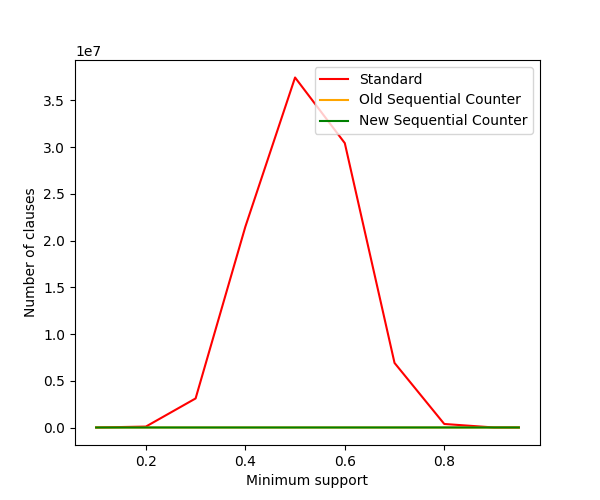
\includegraphics[width=0.8\textwidth]{chapter4/image/n_trans_28_clauses.png}
    \caption{Comparison of the number of clauses in the CNF encoding of the optimization problem using the sequential encounter encodings and the standard encoding.}
    \label{fig:4_1}
\end{figure}

This graph illustrates a notable difference between the number of clauses in the CNF encoding
utilizing the sequential encounter encodings (orange and green line) compared to the standard encoding method (red line).
Particularly, it demonstrates that the sequential encounter encoding results in a significantly smaller number of clauses and variables.

Of special interest is the observation that the number of clauses generated by the standard encoding reaches a peak value,
approximately 35 million clauses, as the minimum support approaches the midpoint threshold.
This suggests a critical point where the standard encoding method generates an overwhelming number of clauses,
highlighting the potential inefficiency and scalability issues associated with this approach.

Additionally, the number of clauses generated by the sequential encounter encoding methods appears to remain consistently low,
maintaining stability across various levels of minimum support.
This suggests that the sequential encounter encoding method is capable of producing fewer clauses while still ensuring the efficiency of the encoding process,
thus keeping the data analysis process manageable even as the constraints grow larger.

In addition to comparing the number of clauses, we also compared the time taken to find all solutions using both methods.
The results are shown in Figure \ref{fig:4_2}.
% figure
\begin{figure}[H]
    \centering
    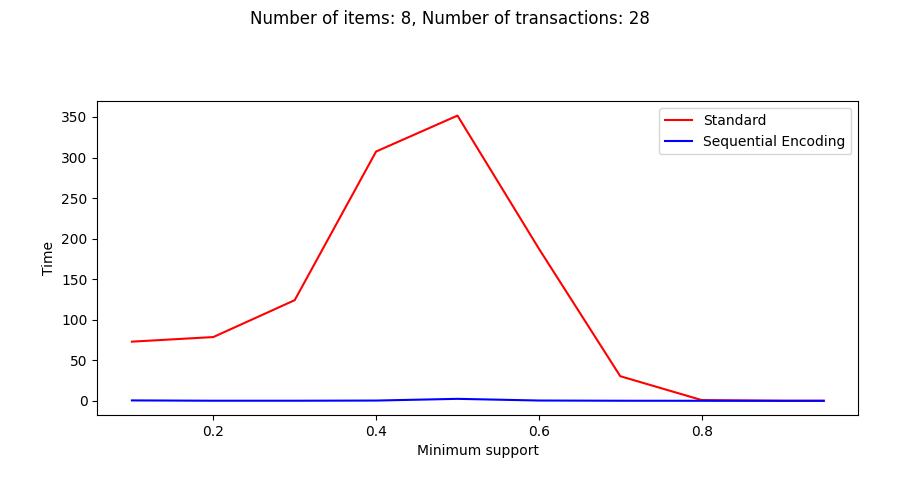
\includegraphics[width=0.8\textwidth]{chapter4/image/n_trans_28_time.png}
    \caption{Comparison of the time taken to find all solutions using the sequential encounter encoding and the standard encodings}
    \label{fig:4_2}
\end{figure}

The graph indicates that the sequential encounter encoding methods consistently outperforms the standard encoding method in terms of time efficiency.
Even as the complexity of the problem increases, the sequential encounter encoding method demonstrates faster solution-finding times,
highlighting its superiority not only in minimizing the number of clauses but also in accelerating the solution discovery process.

However, it's worth noting that while the number of variables may increase, this increment is negligible compared to the significant reduction in the number of clauses.
\begin{figure}[H]
    \centering
    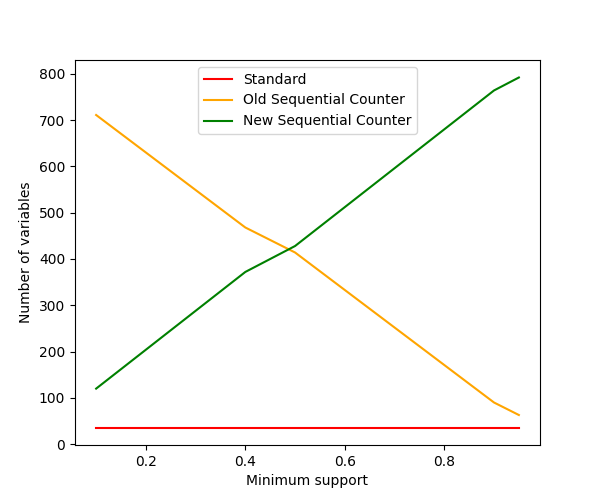
\includegraphics[width=0.8\textwidth]{chapter4/image/n_trans_28_vars.png}
    \caption{Comparison of the number of variables in the CNF encoding of the optimization problem using the sequential encounter encodings and the standard encoding.}
    \label{fig:4_3}
\end{figure}

The graph depicted in Figure \ref{fig:4_3} presents the number of variables in the CNF encoding for each encoding method. It reveals an interesting observation: the old sequential encounter encoding initially has a higher number of variables compared to the standard encoding. However, as the minimum support increases, the number of variables decreases and eventually becomes lower than the standard method. On the other hand, the new sequential counter encoding starts with a lower number of variables, but it gradually increases and surpasses the standard encoding. This indicates a limitation of the new sequential counter encoding method, as it tends to generate a higher number of variables as the minimum support increases.

To further test the performance, we conducted additional experiments. First, we increased the number of transactions from 25 to 28 and compared the number of variables in the CNF encoding of the optimization problem using the sequential encounter encoding and the standard encoding. The results are shown in Figure \ref{fig:4_4}.

Next, we kept the number of transactions constant and varied the minimum support from 0.1 to 0.9 (step 0.1). We then compared the number of variables in the CNF encoding using both encoding methods. The results are shown in Figure \ref{fig:4_5}.

These additional tests provide a more comprehensive evaluation of the sequential encounter encoding method and the standard encoding method, allowing us to assess their performance under different scenarios.

\begin{figure}[H]
    \centering
    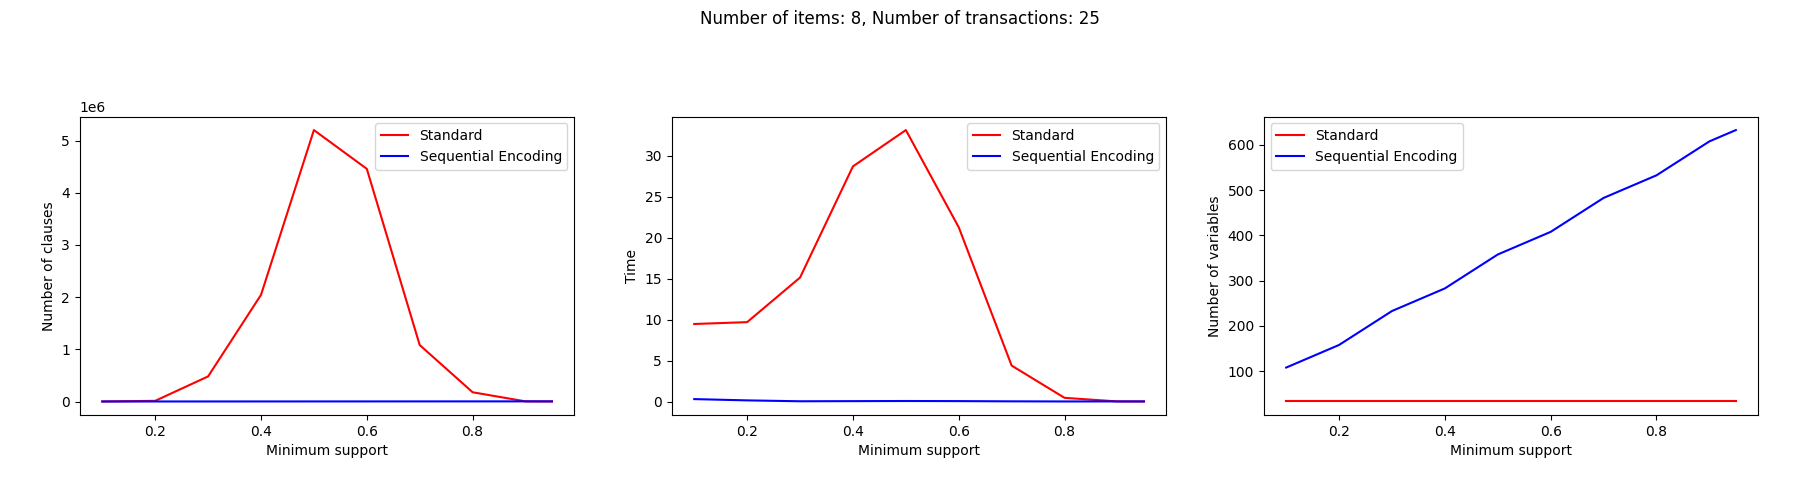
\includegraphics[width=1\textwidth]{chapter4/image/n_trans_25.png}
    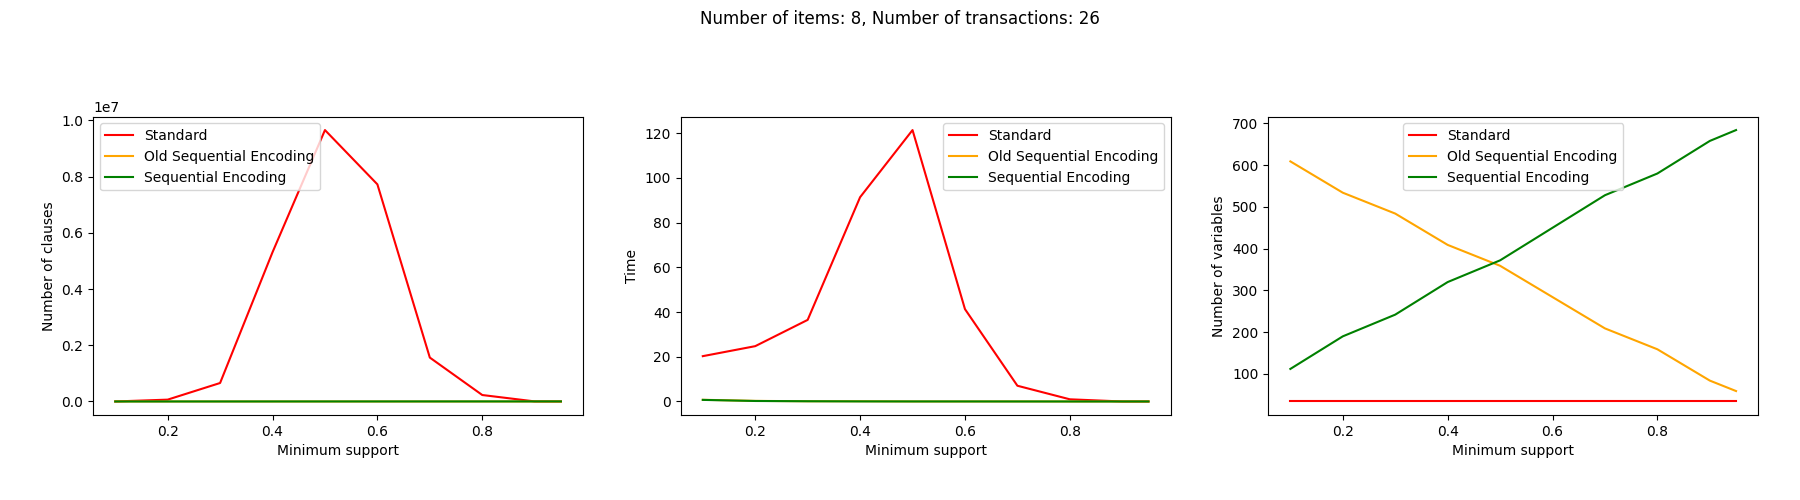
\includegraphics[width=1\textwidth]{chapter4/image/n_trans_26.png}
    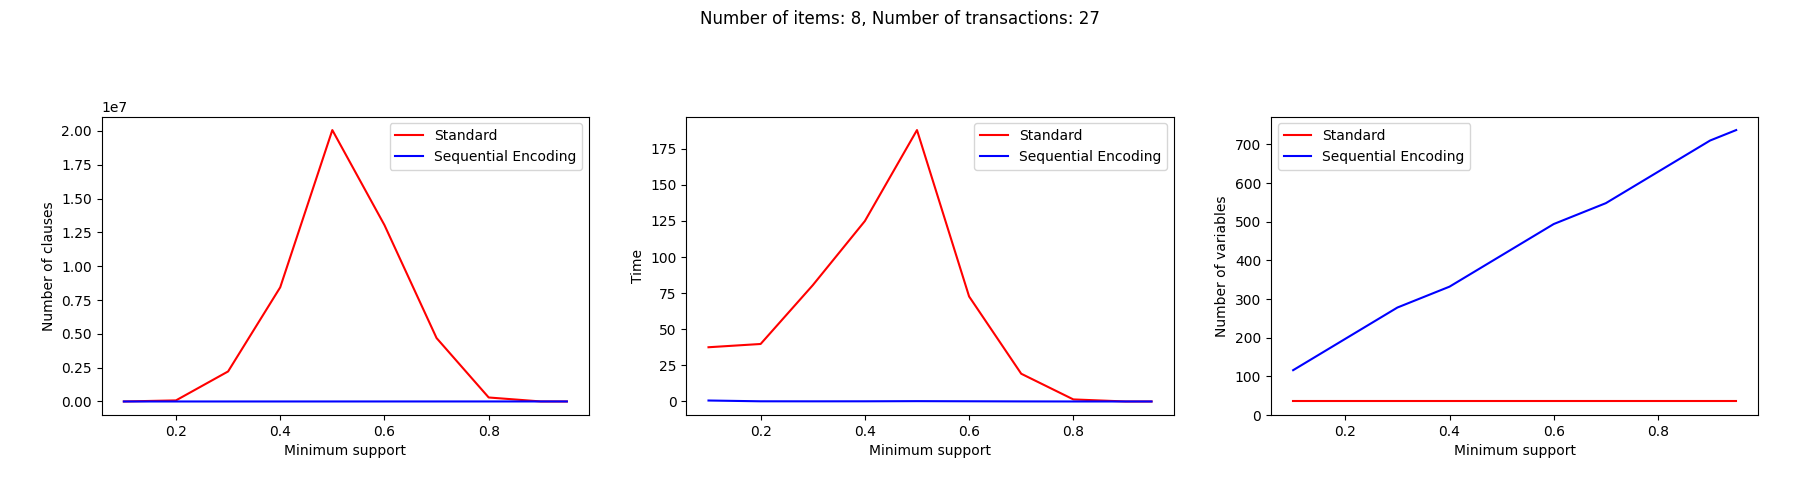
\includegraphics[width=1\textwidth]{chapter4/image/n_trans_27.png}
    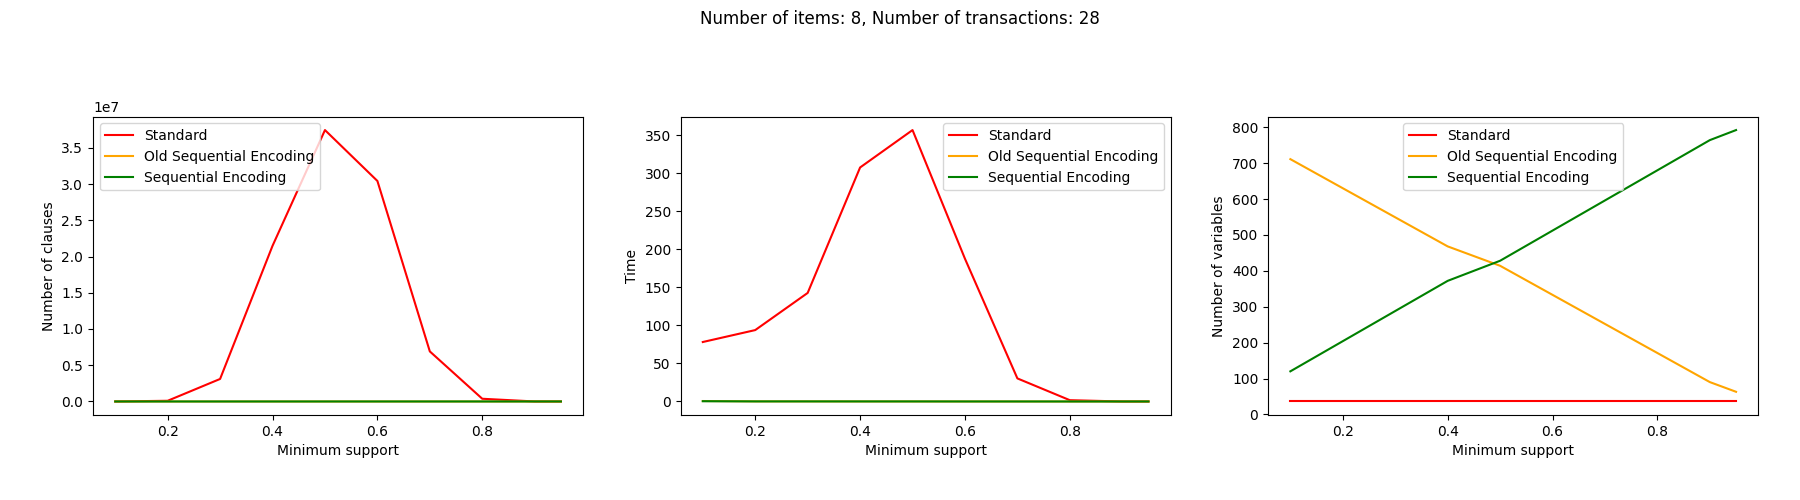
\includegraphics[width=1\textwidth]{chapter4/image/n_trans_28.png}
    \caption{Comparison of the number of variables in the CNF encoding of the optimization problem using the sequential encounter encodings and the standard encoding with other number transactions.}
    \label{fig:4_4}
\end{figure}

\begin{figure}[H]
    \centering
    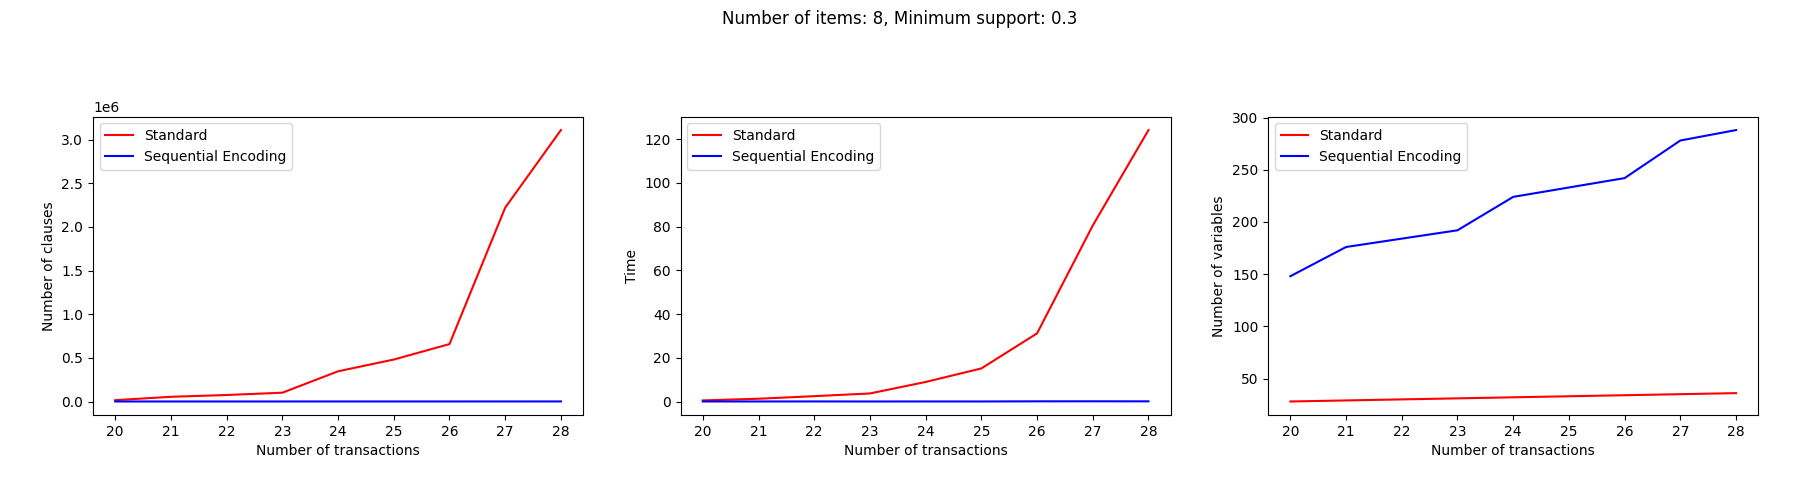
\includegraphics[width=1\textwidth]{chapter4/image/min_supp_0.3.png}
    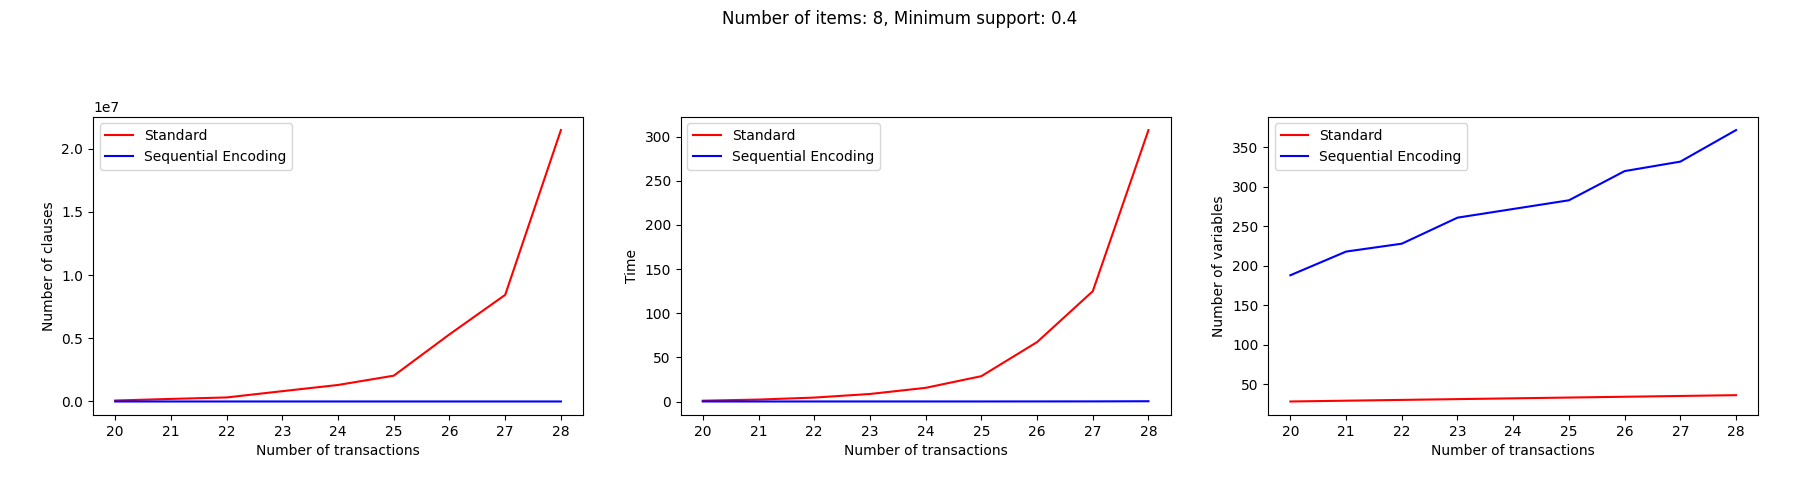
\includegraphics[width=1\textwidth]{chapter4/image/min_supp_0.4.png}
    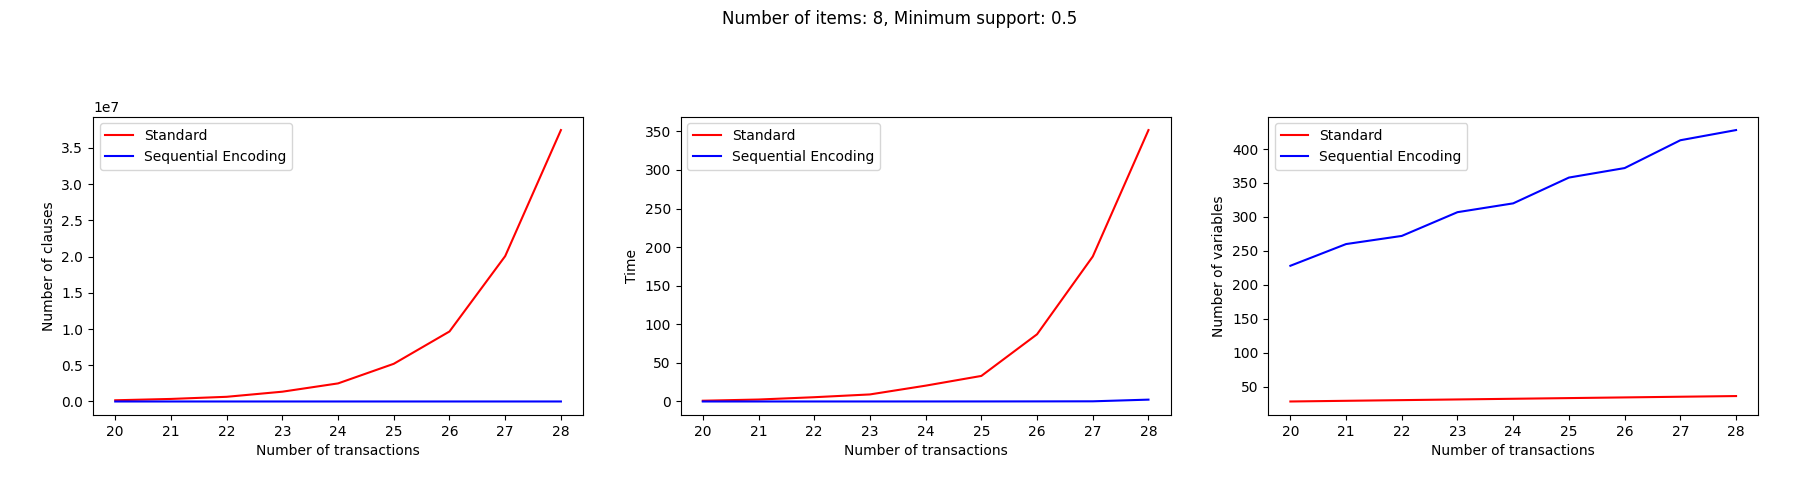
\includegraphics[width=1\textwidth]{chapter4/image/min_supp_0.5.png}
    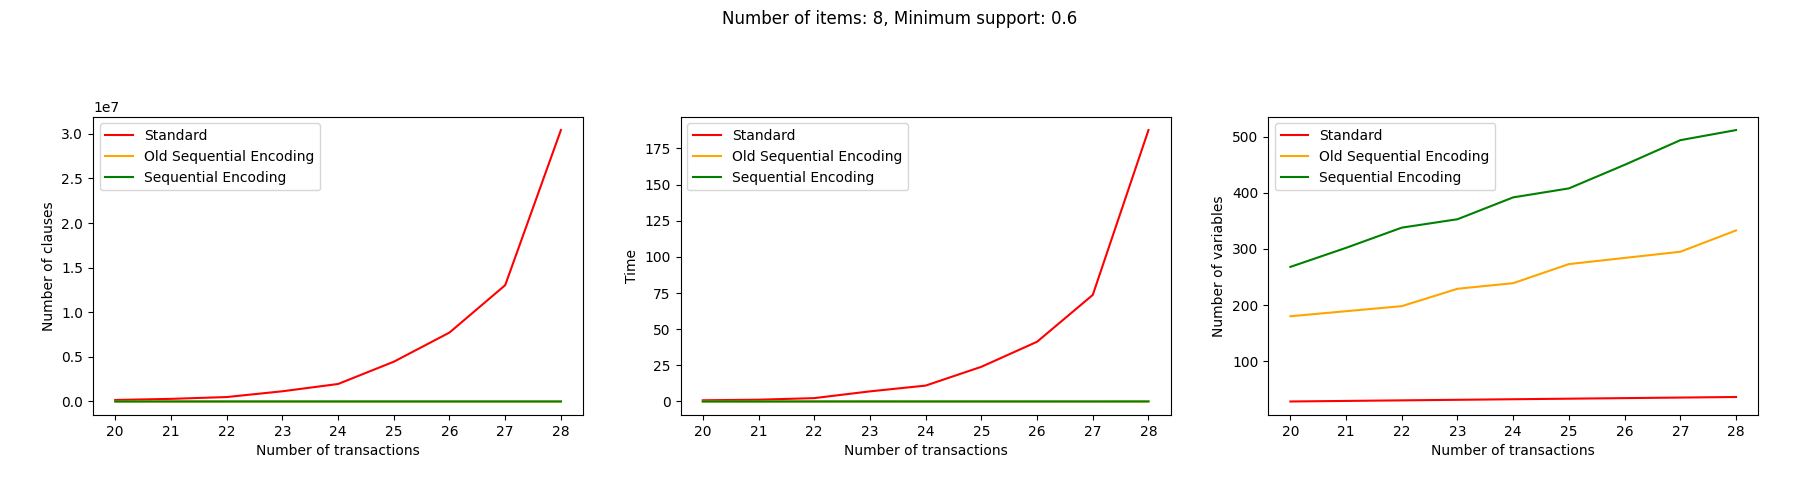
\includegraphics[width=1\textwidth]{chapter4/image/min_supp_0.6.png}
    \caption{Comparison of the number of variables in the CNF encoding of the optimization problem using the sequential encounter encodings and the standard encoding with other minsupp in the same number of transactions.}
    \label{fig:4_5}
\end{figure}

This observation underscores the efficiency of the sequential encounter encoding methods in striking a balance between the complexity of the problem and the computational resources required.
Despite the slight increase in variables, the overall computational overhead remains substantially lower,
making the sequential encounter encoding method a promising approach for tackling large-scale constraint satisfaction problems.

In addition, the experiments were conducted using various combinations of parameters to evaluate the performance of the sequential encounter encoding and the standard encoding in solving the optimization problem. By varying the number of transactions from 26 to 28 and the minimum support from 0.1 to 0.9, we aimed to assess the scalability and efficiency of both encoding methods across different problem sizes and constraints.
\begin{itemize}
    \item Number of items: 8
    \item Number of transactions: 26 to 28
    \item Minimum Support: 0.1 to 0.9
\end{itemize}

Table \ref{tab:4_1} presents the results obtained from these experiments.
It provides a comprehensive comparison of the number of variables, clauses, solutions, and time taken for each combination of parameters using both the standard encoding and the sequential encounter encoding.
\begin{table}[H]
    \centering
    \caption{Comparison of the number of variables, clauses, solutions, and time taken to find all solutions using the sequential encounter encoding methods and the standard encoding method}
    \label{tab:4_1}
    \begin{tabular}{|c|c|r|r|r|r|r|r|r|r|r|}
        \hline
        \multirow{2}{*}{\textbf{Trans}} & \multirow{2}{*}{\textbf{MinSupp}} & \multicolumn{3}{r|}{\textbf{Standard}} & \multicolumn{3}{r|}{\textbf{OSC}} & \multicolumn{3}{r|}{\textbf{NSC}}                                                                                                       \\ \cline{3-11}
                                        &                                   & \textbf{Vars}                          & \textbf{Clauses}                  & \textbf{Time}                     & \textbf{Vars} & \textbf{Clauses} & \textbf{Time} & \textbf{Vars} & \textbf{Clauses} & \textbf{Time} \\ \hline
        25                              & 0.20                              & 33                                     & 12,779                            & 10.46                             & 513           & 1,092            & \textbf{0.15} & 158           & 623              & \textbf{0.15} \\ \hline
        25                              & 0.30                              & 33                                     & 480,829                           & 18.53                             & 441           & 951              & 0.06          & 233           & 929              & \textbf{0.05} \\ \hline
        25                              & 0.40                              & 33                                     & 2,043,104                         & 31.87                             & 393           & 857              & \textbf{0.03} & 283           & 1,138            & 0.05          \\ \hline
        25                              & 0.50                              & 33                                     & 5,200,429                         & 42.30                             & 321           & 716              & \textbf{0.02} & 358           & 1,459            & \textbf{0.02} \\ \hline
        25                              & 0.60                              & 33                                     & 4,457,529                         & 23.99                             & 273           & 622              & \textbf{0.01} & 408           & 1,678            & \textbf{0.01} \\ \hline
        25                              & 0.70                              & 33                                     & 1,081,704                         & 4.72                              & 201           & 481              & \textbf{0.01} & 483           & 2,014            & \textbf{0.01} \\ \hline
        25                              & 0.80                              & 33                                     & 177,229                           & 0.48                              & 153           & 387              & \textbf{0.01} & 533           & 2,243            & \textbf{0.01} \\ \hline
        25                              & 0.90                              & 33                                     & 2,429                             & 0.01                              & 81            & 246              & \textbf{0.01} & 608           & 2,594            & \textbf{0.01} \\ \hline
        25                              & 0.95                              & 33                                     & 429                               & 0.00                              & 57            & 199              & \textbf{0.01} & 633           & 2,713            & \textbf{0.01} \\ \hline
        26                              & 0.10                              & 34                                     & 449                               & 20.26                             & 609           & 1,275            & 0.40          & 112           & 431              & \textbf{0.37} \\ \hline
        26                              & 0.20                              & 34                                     & 65,904                            & 24.73                             & 534           & 1,128            & \textbf{0.10} & 190           & 743              & 0.15          \\ \hline
        26                              & 0.30                              & 34                                     & 657,924                           & 36.48                             & 484           & 1,030            & 0.09          & 242           & 956              & \textbf{0.07} \\ \hline
        26                              & 0.40                              & 34                                     & 5,311,859                         & 91.32                             & 409           & 883              & \textbf{0.02} & 320           & 1,283            & \textbf{0.02} \\ \hline
        26                              & 0.50                              & 34                                     & 9,657,855                         & 121.32                            & 359           & 785              & \textbf{0.01} & 372           & 1,506            & \textbf{0.01} \\ \hline
        26                              & 0.60                              & 34                                     & 7,726,315                         & 41.29                             & 284           & 638              & \textbf{0.01} & 450           & 1,848            & \textbf{0.01} \\ \hline
        26                              & 0.70                              & 34                                     & 1,562,399                         & 7.04                              & 209           & 491              & \textbf{0.01} & 528           & 2,199            & \textbf{0.01} \\ \hline
        26                              & 0.80                              & 34                                     & 230,354                           & 0.98                              & 159           & 393              & \textbf{0.01} & 580           & 2,438            & \textbf{0.01} \\ \hline
        26                              & 0.90                              & 34                                     & 2,724                             & 0.01                              & 84            & 246              & \textbf{0.01} & 658           & 2,804            & \textbf{0.01} \\ \hline
        26                              & 0.95                              & 34                                     & 449                               & 0.00                              & 59            & 197              & \textbf{0.01} & 684           & 2,928            & \textbf{0.01} \\ \hline
        27                              & 0.10                              & 35                                     & 486                               & 41.29                             & 659           & 1,384            & \textbf{0.43} & 116           & 454              & 0.50          \\ \hline
        27                              & 0.20                              & 35                                     & 80,865                            & 44.98                             & 581           & 1,231            & 0.16          & 197           & 778              & \textbf{0.09} \\ \hline
        27                              & 0.30                              & 35                                     & 2,220,210                         & 83.91                             & 503           & 1,078            & \textbf{0.04} & 278           & 1,111            & 0.08          \\ \hline
        27                              & 0.40                              & 35                                     & 8,436,420                         & 160.14                            & 451           & 976              & 0.07          & 332           & 1,338            & \textbf{0.03} \\ \hline
        27                              & 0.50                              & 35                                     & 20,058,448                        & 187.89                            & 373           & 823              & \textbf{0.02} & 413           & 1,686            & \textbf{0.02} \\ \hline
        27                              & 0.60                              & 35                                     & 13,038,043                        & 73.68                             & 295           & 670              & \textbf{0.01} & 494           & 2,043            & \textbf{0.01} \\ \hline
        27                              & 0.70                              & 35                                     & 4,686,973                         & 19.21                             & 243           & 568              & \textbf{0.01} & 548           & 2,286            & \textbf{0.01} \\ \hline
        27                              & 0.80                              & 35                                     & 296,145                           & 0.78                              & 165           & 415              & \textbf{0.01} & 629           & 2,658            & \textbf{0.01} \\ \hline
        27                              & 0.90                              & 35                                     & 3,060                             & 0.01                              & 87            & 262              & \textbf{0.01} & 710           & 3,039            & \textbf{0.01} \\ \hline
        27                              & 0.95                              & 35                                     & 486                               & 0.01                              & 61            & 211              & \textbf{0.01} & 737           & 3,168            & \textbf{0.01} \\ \hline
        28                              & 0.10                              & 36                                     & 523                               & 78.17                             & 711           & 1,496            & 0.56          & 120           & 476              & \textbf{0.34} \\ \hline
        28                              & 0.20                              & 36                                     & 98,425                            & 93.86                             & 630           & 1,337            & 0.27          & 204           & 812              & \textbf{0.22} \\ \hline
        28                              & 0.30                              & 36                                     & 3,108,250                         & 142.69                            & 549           & 1,178            & \textbf{0.07} & 288           & 1,157            & \textbf{0.07} \\ \hline
        28                              & 0.40                              & 36                                     & 21,474,349                        & 307.58                            & 468           & 1,019            & \textbf{0.03} & 372           & 1,511            & 0.04          \\ \hline
        28                              & 0.50                              & 36                                     & 37,442,329                        & 356.74                            & 414           & 913              & \textbf{0.02} & 428           & 1,752            & \textbf{0.02} \\ \hline
        28                              & 0.60                              & 36                                     & 30,421,924                        & 187.64                            & 333           & 754              & \textbf{0.01} & 512           & 2,121            & \textbf{0.01} \\ \hline
        28                              & 0.70                              & 36                                     & 6,907,069                         & 30.33                             & 252           & 595              & \textbf{0.01} & 596           & 2,499            & \textbf{0.01} \\ \hline
        28                              & 0.80                              & 36                                     & 376,885                           & 1.71                              & 171           & 436              & \textbf{0.01} & 680           & 2,886            & \textbf{0.01} \\ \hline
        28                              & 0.90                              & 36                                     & 3,421                             & 0.01                              & 90            & 277              & \textbf{0.01} & 764           & 3,282            & \textbf{0.01} \\ \hline
        28                              & 0.95                              & 36                                     & 523                               & 0.00                              & 63            & 224              & \textbf{0.01} & 792           & 3,416            & \textbf{0.01} \\ \hline
    \end{tabular}
\end{table}

From the table \ref{tab:4_1}, we can observe that as the minimum support increases,
the number of clauses and variables in the CNF encoding generally tends to increase for all encoding methods.
However, the sequential encounter encoding consistently generates a significantly smaller number of clauses and variables compared to the standard encoding.
This reduction in the size of the CNF encoding demonstrates the efficiency and effectiveness of the sequential encounter encoding method in representing the optimization problem.

Furthermore, the table also shows the time taken to find all solutions using each encoding method.
It is evident that the sequential encounter encoding outperforms the standard encoding in terms of time efficiency.
Even as the complexity of the problem increases with higher minimum support values, the sequential encounter encoding method demonstrates faster solution-finding times.
This highlights the advantage of using the sequential encounter encoding method for solving large-scale constraint satisfaction problems.

Overall, the experimental results support the superiority of the sequential encounter encoding methods over the standard encoding method in terms of both the size of the CNF encoding and the time efficiency of finding solutions. These findings validate the effectiveness and scalability of the sequential encounter encoding approach in solving optimization problems with varying problem sizes and constraints.

\subsection{OSC and NSC on Real-World Datasets}

To assess the performance of the Old Sequential Counter (OSC) and New Sequential Counter (NSC) encoding methods, we conducted experiments on real-world datasets. This allowed us to evaluate the strengths and weaknesses of each method in a practical setting.

We delve into the empirical evaluation of the sequential encounter encoding technique within the domain of frequent itemset mining. To ascertain the effectiveness and efficiency of this method, a series of comprehensive experiments were conducted using authentic datasets procured from the Frequent Itemset Mining Implementations (FIMI) and Constraint Programming\cite{constraint_programming} for Itemset Mining (CP4IM) repositories.

The initial step involved an extensive preprocessing phase,
wherein the datasets were meticulously formatted to ensure compatibility with
the encoding algorithms. Subsequent to this preprocessing,
the datasets were encoded using only the sequential encounter encoding because the standard encoding method is not feasible due to the large number of variables and clauses generated.

The datasets selected for the experimental study are succinctly summarized
in Table \ref{tab:result_benchmark_real_datasets}.
The table provides an insightful juxtaposition of key metrics such as the number of variables,
clauses, and the computational time expended for each dataset.

\begin{table}[H]
    \centering
    \caption{Comparison of the number of variables, clauses, solutions, and time taken using the sequential encounter encoding and the standard encoding}
    \label{tab:result_benchmark_real_datasets}
    \begin{tabular}{|l|c|r|r|r|r|r|r|}
        \hline
        \multirow{2}{*}{\textbf{Dataset}} & \multirow{2}{*}{\textbf{MinSupp}} & \multicolumn{3}{r|}{\textbf{Old Sequential Counter}} & \multicolumn{3}{r|}{\textbf{New Sequential Counter}}                                                                        \\ \cline{3-8}
                                          &                                   & \textbf{Vars}                                        & \textbf{Clauses}                                     & \textbf{Time}   & \textbf{Vars} & \textbf{Clauses} & \textbf{Time}   \\ \hline
        zoo-1                             & 0.10                              & 9,134                                                & 19,039                                               & 0.09            & 1,245         & 5,489            & \textbf{0.02}   \\ \hline
        zoo-1                             & 0.90                              & 1,134                                                & 3,119                                                & \textbf{0.01}   & 9,325         & 41,529           & 0.11            \\ \hline
        primary-tumor                     & 0.10                              & 101,536                                              & 206,551                                              & 0.44            & 11,790        & 50,304           & \textbf{0.10}   \\ \hline
        primary-tumor                     & 0.90                              & 11,421                                               & 26,590                                               & \textbf{0.07}   & 102,174       & 455,956          & 0.98            \\ \hline
        vote                              & 0.10                              & 170,168                                              & 343,507                                              & 0.70            & 19,614        & 81,411           & \textbf{0.17}   \\ \hline
        vote                              & 0.90                              & 19,136                                               & 41,791                                               & \textbf{0.11}   & 170,994       & 761,229          & 1.54            \\ \hline
        soybean                           & 0.10                              & 357,313                                              & 718,627                                              & 1.64            & 40,360        & 165,745          & \textbf{0.36}   \\ \hline
        soybean                           & 0.90                              & 40,297                                               & 85,099                                               & \textbf{0.21}   & 357,880       & 1,592,317        & 3.45            \\ \hline
        chess                             & 0.10                              & 9,192,090                                            & 18,450,064                                           & 42.33           & 1,025,990     & 4,212,750        & \textbf{9.45}   \\ \hline
        chess                             & 0.20                              & 8,169,690                                            & 16,405,584                                           & 37.10           & 2,048,710     & 8,455,790        & \textbf{18.16}  \\ \hline
        chess                             & 0.80                              & 2,044,875                                            & 4,157,871                                            & \textbf{10.75}  & 8,175,442     & 36,018,416       & 82.85           \\ \hline
        chess                             & 0.90                              & 1,022,475                                            & 2,113,391                                            & \textbf{6.32}   & 9,198,162     & 40,977,296       & 109.49          \\ \hline
        mushroom                          & 0.10                              & -                                                    & -                                                    & -               & 6,613,018     & 26,853,806       & \textbf{65.64}  \\ \hline
        mushroom                          & 0.20                              & -                                                    & -                                                    & -               & 13,209,706    & 54,226,732       & \textbf{187.69} \\ \hline
        mushroom                          & 0.30                              & -                                                    & -                                                    & -               & 19,814,518    & 82,293,931       & \textbf{798.24} \\ \hline
        mushroom                          & 0.40                              & 39,599,708                                           & 79,293,980                                           & \textbf{212.00} & -             & -                & -               \\ \hline
        mushroom                          & 0.50                              & 33,003,832                                           & 66,103,040                                           & \textbf{155.02} & -             & -                & -               \\ \hline
        mushroom                          & 0.60                              & 26,399,833                                           & 52,895,855                                           & \textbf{136.33} & -             & -                & -               \\ \hline
        mushroom                          & 0.70                              & 19,803,957                                           & 39,704,915                                           & \textbf{237.99} & -             & -                & -               \\ \hline
        mushroom                          & 0.80                              & 13,199,958                                           & 26,497,730                                           & \textbf{62.56}  & -             & -                & -               \\ \hline
        mushroom                          & 0.90                              & 6,604,082                                            & 13,306,790                                           & \textbf{29.05}  & -             & -                & -               \\ \hline
    \end{tabular}
\end{table}

The results in Table \ref{tab:result_benchmark_real_datasets} provide a comprehensive overview of the performance of the sequential encounter encoding methods on real-world datasets.
These experiments demonstrate that the Old Sequential Counter (OSC) encoding method is more efficient than the New Sequential Counter (NSC) encoding method when the minimum support is larger.
Conversely, NSC is more efficient than OSC when the minimum support is smaller.
The strong evident is with the mushroom dataset, only the NSC encoding method can solve the problem when the minimum support is set to 0.1, 0.2, and 0.3. Conversely, only the OSC encoding method can solve the problem when the minimum support is set to 0.4, 0.5, 0.6, 0.7, 0.8, and 0.9. By combining both the OSC and NSC methods, the problem can be solved for all minimum support values.

Observing Table \ref{tab:result_benchmark_real_datasets}, it becomes evident
that the sequential encounter encoding method demonstrates varied performance benefits across different datasets.
For instance, the 'zoo-1' dataset, characterized by 36 items and 101 transactions,
was encoded with significantly fewer variables and clauses, resulting in an impressively swift computation time of
only 0.02 seconds. And with $MinSupp$ increase to 0.9, by OSC, it take only 0.01 to resolve.
This marked efficiency showcases the potential of the sequential encounter encoding in dealing with
smaller datasets.

Conversely, as we scrutinize datasets with a larger number of transactions and items,
such as 'chess' and 'mushroom', we notice a discernible trend of increased complexity.
The 'chess' dataset at a 0.10 minimum support level demanded over a million variables in the standard encoding approach,
with a consequent computational time of approximately 9.45 seconds by NSC
and 6.32 seconds by OSC when the minimum support is increased to 0.90.
The escalation in complexity is palpable when the minimum support is altered,
impacting the number of solutions and, inevitably, the time required for computation.

The 'mushroom' dataset provides additional insights into the scalability issues.
For the NSC, the number of variables reaches its peak at a minimum support of 0.30, resulting in a significant computational time of 798.24 seconds.
However, OSC is unable to resolve this dataset. As the minimum support increases, OSC becomes the only viable option and demonstrates improved performance.
The number of variables and clauses decrease, and the computational time also decreases significantly, leading to better results.
This starkly contrasts with the lesser demanding 'zoo-1' and 'primary-tumor' datasets,
underscoring the necessity of an encoding method that can adeptly adapt to varying dataset sizes and complexities.

In summary, the experimental evaluation substantiates the hypothesis that sequential encounter encoding can be a potent alternative to standard encoding in itemset mining,
particularly when tailored to the dataset at hand.
Beside that, the new sequential counter encoding method is more efficient than the old sequential counter encoding method when the minimum support is smaller, and vice versa.
By combining both methods, the problem can be solved for all minimum support values.
